\documentclass[tikz,border=8pt]{standalone}
\usepackage[T1]{fontenc}
\usepackage{helvet}
\renewcommand{\familydefault}{\sfdefault}
\usepackage{amsmath}
\usepackage{xcolor}
\usetikzlibrary{arrows.meta, positioning}

\definecolor{ink}{HTML}{1F2937}
\definecolor{blueA}{HTML}{E8F1FB}
\definecolor{blueB}{HTML}{2F6B9A}
\definecolor{tealA}{HTML}{E7F7F5}
\definecolor{tealB}{HTML}{1D8B74}
\definecolor{orangeA}{HTML}{FFF1E6}
\definecolor{orangeB}{HTML}{C86A1A}
\definecolor{greenA}{HTML}{EAF7E9}
\definecolor{greenB}{HTML}{2E7D32}
\definecolor{redA}{HTML}{FDECEC}
\definecolor{redB}{HTML}{B23A3A}
\definecolor{grayB}{HTML}{5B6470}

\tikzset{
  title/.style={font=\bfseries\fontsize{24}{26}\selectfont, text=ink},
  subtitle/.style={font=\bfseries\fontsize{15}{17}\selectfont, text=ink},
  body/.style={font=\fontsize{11}{13}\selectfont, text=ink},
  smallbody/.style={font=\fontsize{10}{12}\selectfont, text=ink},
  box/.style={rounded corners=14pt, draw=grayB!35, line width=1.1pt, fill=white, inner sep=12pt, align=left},
  bluebox/.style={box, fill=blueA},
  tealbox/.style={box, fill=tealA},
  orangebox/.style={box, fill=orangeA},
  greenbox/.style={box, fill=greenA},
  redbox/.style={box, fill=redA}
}
\newcommand{\subtitle}{\bfseries\fontsize{15}{17}\selectfont\color{ink}}
\newcommand{\body}{\fontsize{11}{13}\selectfont\color{ink}}
\newcommand{\smallbody}{\fontsize{10}{12}\selectfont\color{ink}}

\begin{document}
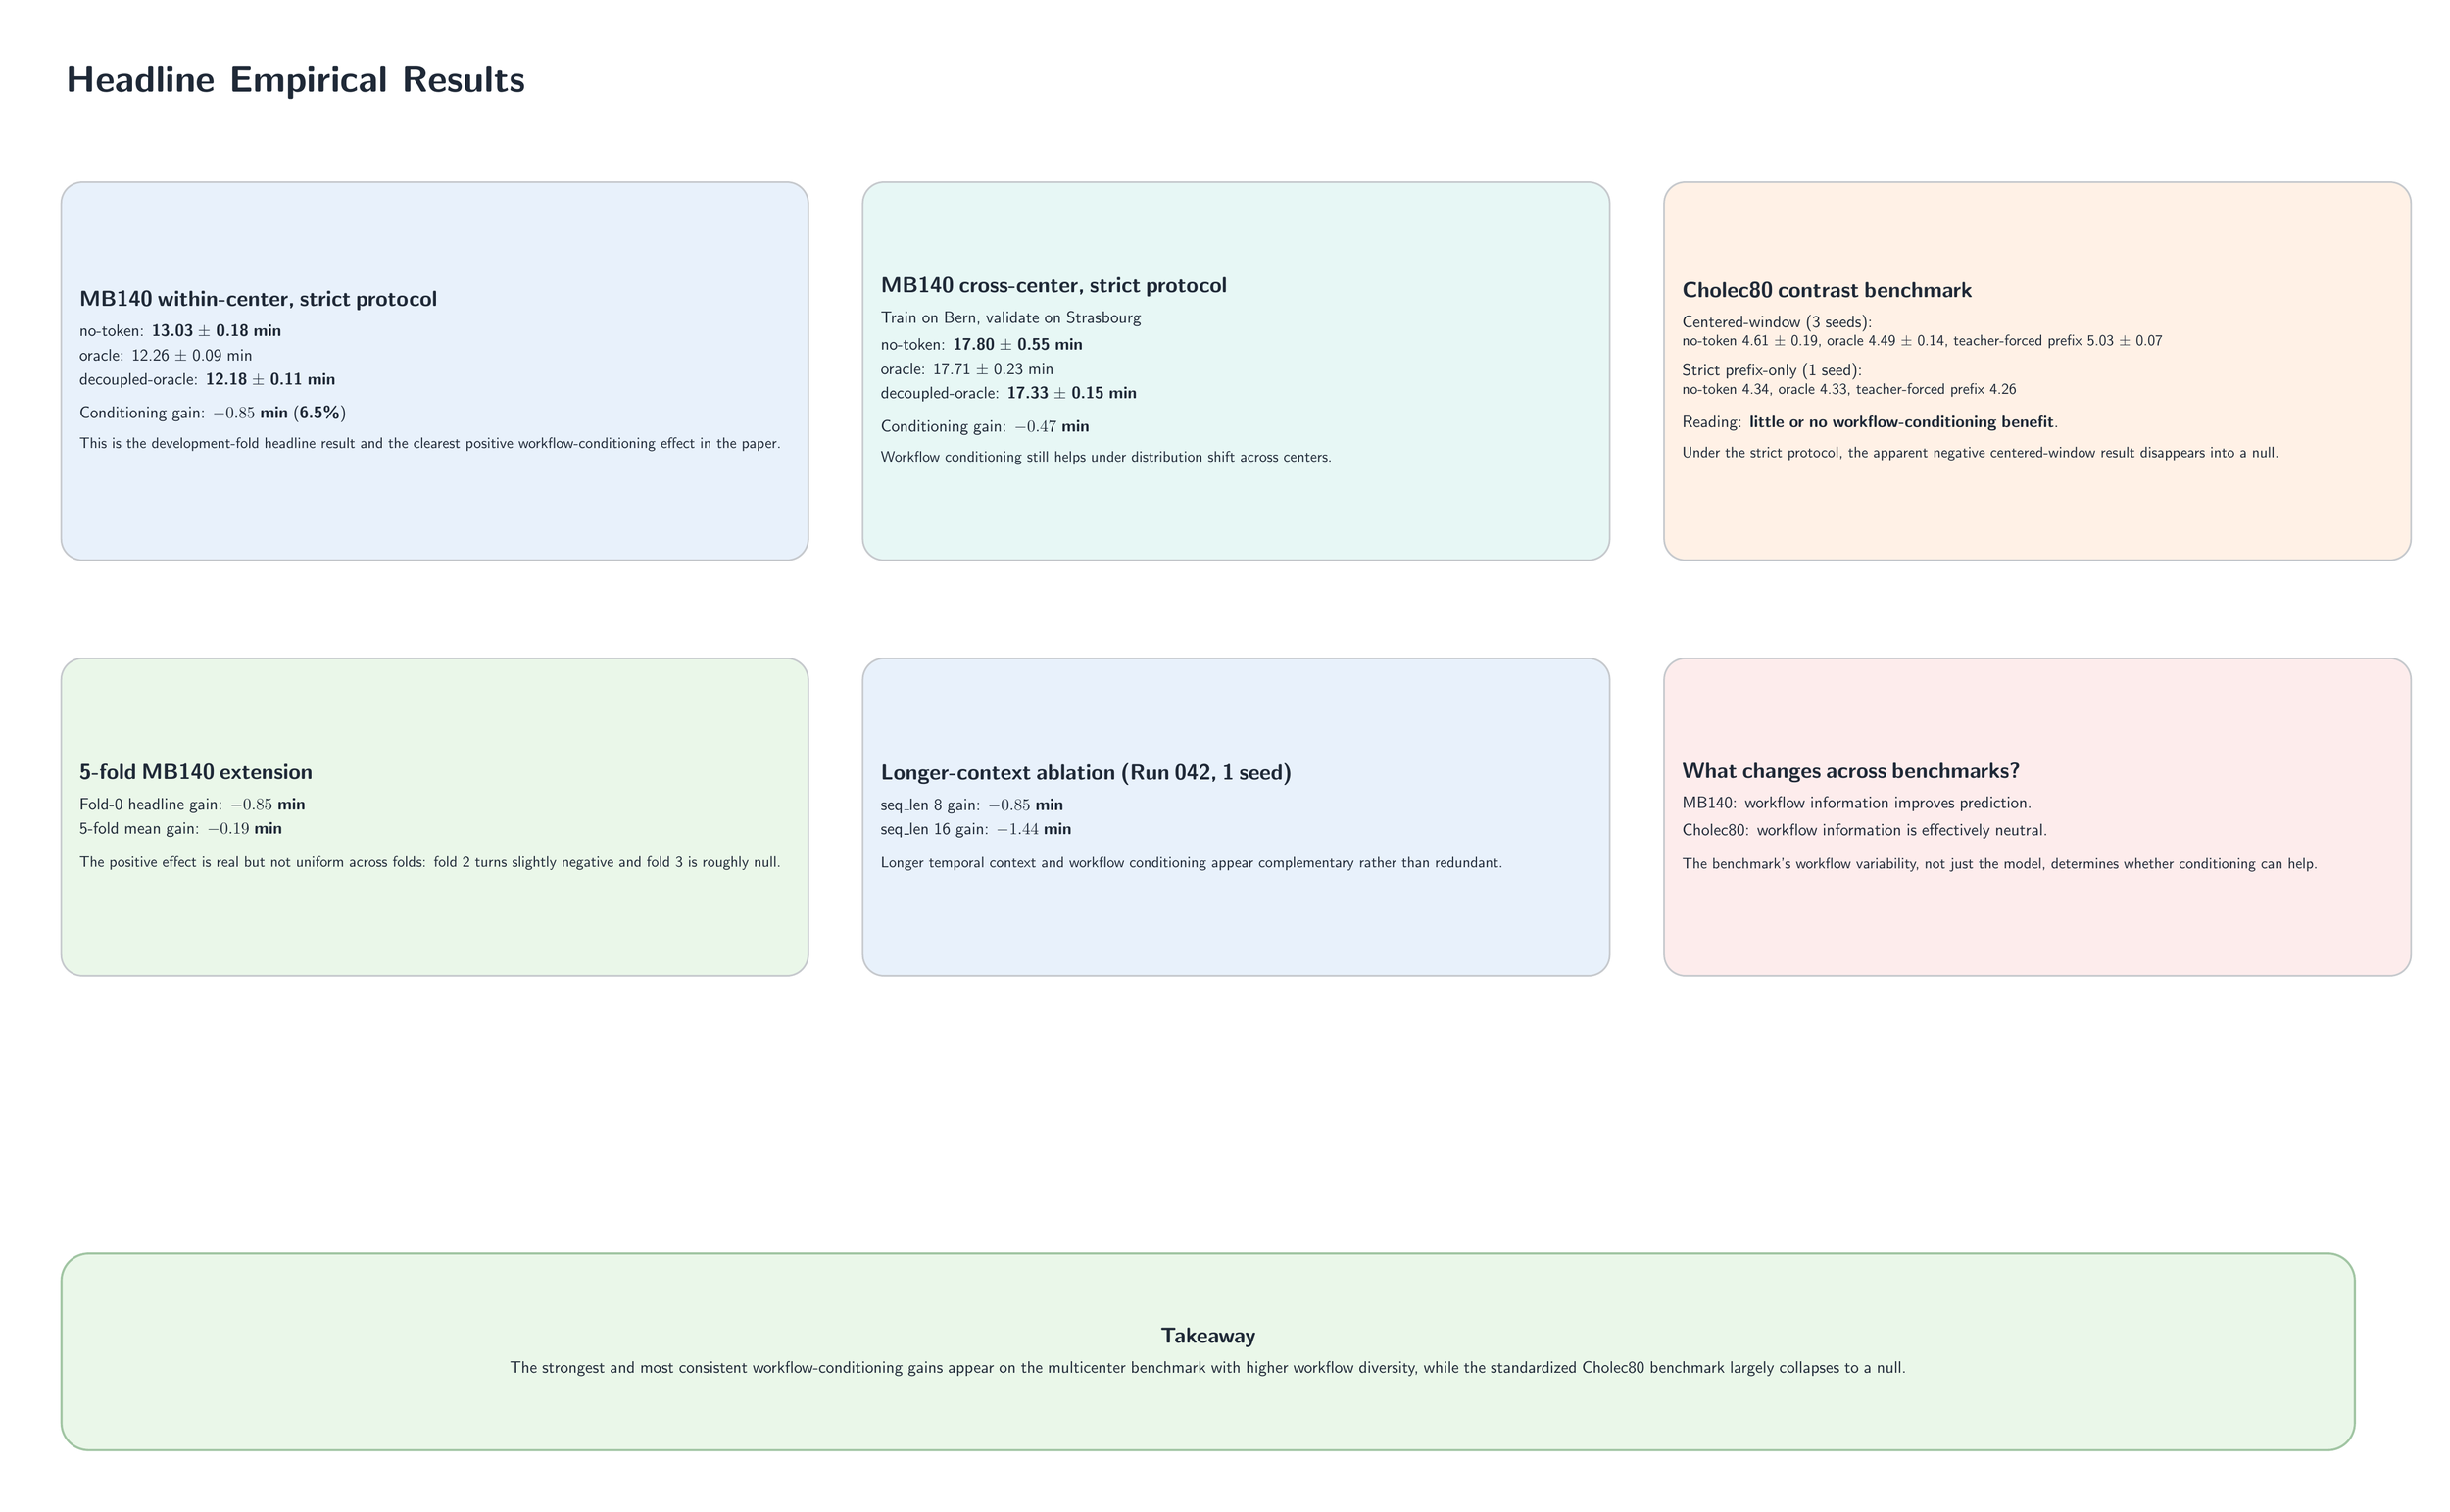
\begin{tikzpicture}[x=1pt,y=1pt]
\useasboundingbox (0,0) rectangle (1600,980);

\node[title, anchor=north west] at (30,950)
{Headline Empirical Results};

\node[bluebox, text width=470pt, minimum height=250pt, anchor=north west] at (30,870) {
{\subtitle MB140 within-center, strict protocol}\par\vspace{8pt}
{\body no-token: \textbf{13.03 \(\pm\) 0.18 min}}\par\vspace{4pt}
{\body oracle: 12.26 \(\pm\) 0.09 min}\par\vspace{4pt}
{\body decoupled-oracle: \textbf{12.18 \(\pm\) 0.11 min}}\par\vspace{10pt}
{\body Conditioning gain: \textbf{\(-0.85\) min} (\textbf{6.5\%})}\par\vspace{8pt}
{\smallbody This is the development-fold headline result and the clearest positive workflow-conditioning effect in the paper.}
};

\node[tealbox, text width=470pt, minimum height=250pt, anchor=north west] at (560,870) {
{\subtitle MB140 cross-center, strict protocol}\par\vspace{8pt}
{\body Train on Bern, validate on Strasbourg}\par\vspace{6pt}
{\body no-token: \textbf{17.80 \(\pm\) 0.55 min}}\par\vspace{4pt}
{\body oracle: 17.71 \(\pm\) 0.23 min}\par\vspace{4pt}
{\body decoupled-oracle: \textbf{17.33 \(\pm\) 0.15 min}}\par\vspace{10pt}
{\body Conditioning gain: \textbf{\(-0.47\) min}}\par\vspace{8pt}
{\smallbody Workflow conditioning still helps under distribution shift across centers.}
};

\node[orangebox, text width=470pt, minimum height=250pt, anchor=north west] at (1090,870) {
{\subtitle Cholec80 contrast benchmark}\par\vspace{8pt}
{\body Centered-window (3 seeds):}\par
{\smallbody no-token 4.61 \(\pm\) 0.19, oracle 4.49 \(\pm\) 0.14, teacher-forced prefix 5.03 \(\pm\) 0.07}\par\vspace{8pt}
{\body Strict prefix-only (1 seed):}\par
{\smallbody no-token 4.34, oracle 4.33, teacher-forced prefix 4.26}\par\vspace{10pt}
{\body Reading: \textbf{little or no workflow-conditioning benefit}.}\par\vspace{8pt}
{\smallbody Under the strict protocol, the apparent negative centered-window result disappears into a null.}
};

\node[greenbox, text width=470pt, minimum height=210pt, anchor=north west] at (30,555) {
{\subtitle 5-fold MB140 extension}\par\vspace{8pt}
{\body Fold-0 headline gain: \textbf{\(-0.85\) min}}\par\vspace{4pt}
{\body 5-fold mean gain: \textbf{\(-0.19\) min}}\par\vspace{10pt}
{\smallbody The positive effect is real but not uniform across folds: fold 2 turns slightly negative and fold 3 is roughly null.}
};

\node[bluebox, text width=470pt, minimum height=210pt, anchor=north west] at (560,555) {
{\subtitle Longer-context ablation (Run 042, 1 seed)}\par\vspace{8pt}
{\body seq\_len 8 gain: \textbf{\(-0.85\) min}}\par\vspace{4pt}
{\body seq\_len 16 gain: \textbf{\(-1.44\) min}}\par\vspace{10pt}
{\smallbody Longer temporal context and workflow conditioning appear complementary rather than redundant.}
};

\node[redbox, text width=470pt, minimum height=210pt, anchor=north west] at (1090,555) {
{\subtitle What changes across benchmarks?}\par\vspace{8pt}
{\body MB140: workflow information improves prediction.}\par\vspace{6pt}
{\body Cholec80: workflow information is effectively neutral.}\par\vspace{10pt}
{\smallbody The benchmark's workflow variability, not just the model, determines whether conditioning can help.}
};

\node[rounded corners=18pt, draw=greenB!45, fill=greenA, line width=1.4pt, text width=1510pt, minimum height=130pt, align=center, anchor=south west] at (30,30) {
{\subtitle Takeaway}\par\vspace{8pt}
{\body The strongest and most consistent workflow-conditioning gains appear on the multicenter benchmark with higher workflow diversity, while the standardized Cholec80 benchmark largely collapses to a null.}
};

\end{tikzpicture}
\end{document}
